\subsubsection{Model Evaluation}
	\paragraph{Classification Error \& Confusion Matrix}
		\RTheory
		{
			$$\varepsilon = \frac{1}{N}\sum\limits_{n = 0}^N I(\hat{y}_n \neq y_n)$$
			
			\vspace{0pt}
			
			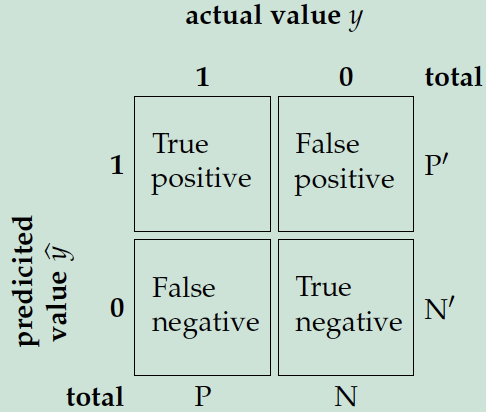
\includegraphics[scale=0.5]{images/ConfusionMatrix.png}
		}
		{
			sections/Classification/LogisticRegression/ModelEvaluation/ClassificationError.R
		}
		
	\paragraph{Cross Validation}
		Generic method for estimating the classification error without needing extra data.
		
		Cross validation is used in order to evaluate the kind of model that is used, not for building it.	 The final model will be built on all of the data.
		 
		\subparagraph{Algorithm}
			\RTheory
			{
				\begin{itemize}
				    \item The \underline{training data} is divided in $k$ groups (folds) of approximately the same size
				    \item First fold is treated as validation set
				    \item The model is fit on the remaining $k-1$ folds
				    \item The classification error $\mathrm{Err}_1$ is calculated
				    \item The process is repeated for the remaining sets, resulting in classification errors $\mathrm{Err}_1, \dots, \mathrm{Err}_k$
				    \item The CV error is computed as: $CV_{(k)} = \frac{1}{k} \sum\limits_{i=1}^k\mathrm{Err}_i$
				\end{itemize}
			}
			{
				sections/Classification/LogisticRegression/ModelEvaluation/CrossValidation.R
			}

		